\documentclass[a4paper, 10pt, final, garamond]{book}
\usepackage{cours-preambule}
\graphicspath{{./figures/}}

\makeatletter
\renewcommand{\@chapapp}{Contr\^ole de connaissances}
\makeatother

% \toggletrue{student}
\toggletrue{corrige}
\renewcommand{\mycol}{black}
% \renewcommand{\mycol}{gray}

\begin{document}
\setcounter{chapter}{24}

\settype{enon}
\settype{solu}

\chapter{Introduction à la thermodynamique\ifstudent{~(13')}}

\begin{enumerate}[label=\sqenumi]
	\item[n]{8}%
	Donner la définition de la température cinétique en
	fonction du degré de liberté $D$. Déterminer alors l'énergie interne d'un
	gaz parfait mono- puis diatomique en fonction de $R$ qu'on reliera à deux
	autres constantes. En déduire les capacités thermiques $C_{V,\rm
				mono}\sup{G.P.}$ et $C_{V,\rm dia}\sup{G.P.}$
	\smallbreak
	\begin{isd}
		\psw{%
			Soit un gaz parfait de $N$ molécules, $D$ le nombre de degrés de liberté~:
			\vspace{-10pt}
			\begin{gather*}
				\moy{e_{c,i}}  D \times \frac{1}{2}k_B T ~ \pt{1}
			\end{gather*}
			\begin{itemize}
				\item[b]{Monoatomique} $\Ra D = 3$ car 3 translations $x,y,z$~;
				\item[b]{Diatomique} $\Ra D = 5$ \pt{1} car 3 translations $x,y,z$ + 2 rotations~;
			\end{itemize}
			\begin{DispWithArrows*}
				U = e_c &= \sum_i \moy{e_{c,i}} \stm{=} \frac{D}{2} Nk_bT
				\Arrow{$N = n \Nc_A$}
				\\\Lra
				U &= \frac{D}{2} n \underbracket[1pt]{\Nc_Ak_B}_{=R \pt{1}} T
			\end{DispWithArrows*}
		}%
		\vspace{-15pt}
		\tcblower
		\begin{center}
			\sswitch{
				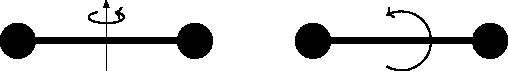
\includegraphics[scale=1, draft=true]{deglib_dia}
			}{
				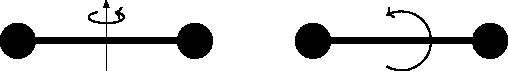
\includegraphics[scale=1]{deglib_dia}
			}
			\vspace{-15pt}
			\captionof{figure}{Degrés de libertés gaz diatomique\protect\pt{1}.}
		\end{center}
		\psw{%
			\begin{DispWithArrows*}
				\Lra
				\boxed{U\ind{mono} = \frac{3}{2}nRT}
				\qMalg{\stk{et}}
				\boxed{U\ind{dia} = \frac{5}{2}nRT}
				\Arrow{$C_V \stm{=} \DS\pdv{U}{T}$}
				\\
				\Ra
				\boxed{C_{V,\rm mono} = \frac{3}{2}nR}
				\qMalg{\stk{et}}
				\boxed{C_{V,\rm dia} = \frac{5}{2}nR}
			\end{DispWithArrows*}
		}%
		\vspace{-15pt}
	\end{isd}
	\item[n]{12}%
	~
	\smallbreak
	\vspace*{-25pt}
	\begin{isd}[righthand ratio=.30, interior hidden]
		On fait subir à $\SI{1}{mol}$ de gaz parfait le cycle mécaniquement
		réversible suivant~:
		\begin{enumerate}[label=\clalphi]
			\item $P_A$ et $V_A$;
			\item Chauffage isochore, $P_B = 2P_A$~;
			\item Détente isotherme quasi-statique, $V_C = 2V_B$~;
			      \item[cl](A) Refroidissement isobare, on retourne à l'état initial.
		\end{enumerate}
		\tcblower
		\begin{center}
			\sswitch{
				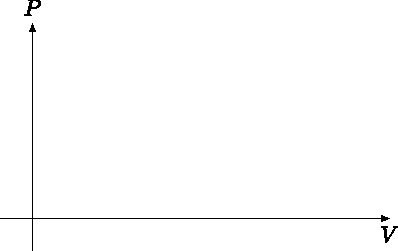
\includegraphics[width=\linewidth, valign=t]{cycle_lenoir-plain}
			}{
				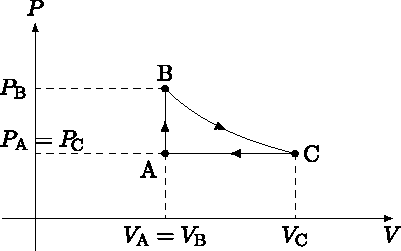
\includegraphics[width=\linewidth, valign=t]{cycle_lenoir}
			}
			\captionof*{figure}{Cycle de \textsc{Lenoir}.~\protect\pt{1}+\protect\pt{1}}
		\end{center}
		\vspace{-30pt}
	\end{isd}
	\begin{enumerate}[label=\sqenumi]
		\item Tracer ce cycle dans le diagramme de \textsc{Watt}. Déterminer la
		      nature du cycle (moteur ou récepteur).
		      % \item Calculer la pression, le volume et la température pour chacun des
		      %       états $A$, $B$ et $C$.
		\item Exprimer sans démonstration le travail infinitésimal des forces de
		      pression. Donner sans démonstration l'expression de $W_p$ dans les cas
		      isochore et monobare. Démontrer l'expression de $W_p$ pour une
		      transformation quasi-statique et isotherme à $T = T_0$ en fonction des
		      volumes $V_i$ et $V_f$.
		\item Exprimer les travaux associés à chaque transformation puis celui du
		      cycle. Simplifier les expressions en analysant les relations entre
		      les volumes.
	\end{enumerate}
	\smallbreak
	\begin{enumerate}[label=\sqenumi]
		\item \psw{Pour la nature, on voit que le cycle s'effectue en \textbf{sens
				      horaire}, donc $W_{p,\rm cycle} < 0$ donc \textbf{moteur}}. \pt{1}
		      % \item
		      %       \begin{enumerate}[label=\clalphi]
		      % 	      \item \psw{%
		      % 		            On a déjà $P_A$ et $V_A$, on cherche $T_A$~:
		      % 		            \[
		      % 			            \boxed{T_A = \frac{P_AV_A}{nR}}
		      % 			            \Ra
		      % 			            \xul{T_A = \SI{337}{K}}
		      % 			            \qav
		      % 			            \left\{
		      % 			            \begin{array}{rcl}
		      % 				            P_A & = & \SI{2e5}{Pa}
		      % 				            \\
		      % 				            V_A & = & \SI{1.4e-2}{m^3}
		      % 				            \\
		      % 				            n   & = & \SI{1}{mol}
		      % 				            \\
		      % 				            R   & = & \SI{8.314}{J.K^{-1}.mol^{-1}}
		      % 			            \end{array}
		      % 			            \right.
		      % 		            \]
		      % 	            }%
		      % 	      \item \psw{%
		      % 		            On connaît $P_B$ et transformation isochore donc
		      % 		            $\boxed{V_B = V_A}$, on cherche $T_B$~:
		      % 		            \[
		      % 			            \boxed{T_B = \frac{P_BV_B}{nR}}
		      % 			            \Ra
		      % 			            \xul{T_B = \SI{674}{K}}
		      % 		            \]
		      % 	            }%
		      % 	      \item \psw{%
		      % 		            On connaît $V_C = 2V_B$ et transformation isotherme donc
		      % 		            $\boxed{T_C = \SI{674}{K}}$, on cherche
		      % 		            $P_C$~:
		      % 		            \[
		      % 			            \boxed{P_C = \frac{nRT_C}{V_C}}
		      % 			            \Ra
		      % 			            \xul{P_C = \SI{2e5}{Pa}}
		      % 		            \]
		      % 	            }%
		      %       \end{enumerate}
		\item[m] \psw{%
				\begin{gather*}
					\delta W_p = -P\ind{ext}\dd{V} \pt{1}
					\quad \Lra \quad
					\delta W_{p,\rm isoV} = 0
					\qMath{et \pt{1}}
					W_p = \int \delta W_p = -P\ind{ext}\Delta{V}
					\\\beforetext{$P = P\ind{ext}$ et $T = T_0 \pt{1} \Ra$}
					W_p =
					- \int_{V_i}^{V_f}P \dd{V} =
					-\int_{V_i}^{V_f} \frac{nRT_0}{V}\dd{V} \pt{1}
					\\\Lra
					W_p = -nRT_0 (\ln V_f - \ln V_i)
					\Lra
					\boxed{W_p \stm{=} nRT_0 \ln (\frac{V_i}{V_f})}
				\end{gather*}
			}%
			\vspace*{\fill}
		\item \begin{itemize}
			      \item
			            \leftcenters{%
				            \psw{%
					            AB~: transformation isochore, donc
				            }%
			            }{%
				            \psw{%
					            $\boxed{W_{p,\rm AB} = 0}$ \pt{1}
				            }%
			            }%
			      \item
			            \leftcenters{%
				            \psw{%
					            BC~: isoT et Q.S. donc
				            }%
			            }{%
				            \psw{%
					            $
						            W_{p,\rm BC} = nRT_B \ln (\frac{V_B}{V_C})
						            \Lra
						            \boxed{W_{p,\rm BC} = -nRT_B \ln 2}~\pt{1}
						            % \Ra
						            % \xul{W_{p,BC} = \SI{-3.88}{kJ}}
					            $
				            }%
			            }%
			      \item
			            \leftcenters{%
				            \psw{%
					            CA~: isobare, donc
				            }%
			            }{%
				            \psw{%
					            $
						            W_{p,\rm CA} = P_C (V_C - V_A)
						            \Lra
						            \boxed{W_{p,\rm CA} = 2P_AV_A}~\pt{1}
						            % \Ra
						            % \xul{W_{p,CA}= \SI{2.8}{kJ}}
					            $
				            }%
			            }%
			      \item
			            \leftcenters{%
				            \psw{%
					            Cycle~:
				            }%
			            }{%
				            \psw{%
					            $\DS
						            W_{p,\rm cycle} = \sum_i W_i = W_{AB} + W_{BC} + W_{CA} =
						            2P_AV_A - nRT_B \ln 2~\pt{1}
					            $
					            % \SI{-1.08}{kJ}
				            }%
			            }%
		      \end{itemize}
	\end{enumerate}
	\vspace{-15pt}
	\ifstudent{
		\begin{tikzpicture}[remember picture, overlay]
			\node[anchor=north west, align=left]
			at ([shift={(1.4cm,0)}]current page.north west)
			{\\[5pt]\Large\bfseries Nom~:\\[10pt]\Large\bfseries Prénom~:};
			\node[anchor=north east, align=right]
			at ([shift={(-1.5cm,-17pt)}]current page.north east)
			{\Large\bfseries Note~:\hspace{1cm}/20};
		\end{tikzpicture}
	}
\end{enumerate}
\end{document}
